\section{Analysis}\label{sc:analysis}
In order to asses the correct progress of the rnucs-mesh workflow, a few 
analysis were performed on toy problems designed to have interaction in the 
high energy region. 

\subsection{Problem Description}
Two toy problems were identified to asses the correctness of the 
rnucs-mesh workflow. 
Toy problem I (shown in Figure \ref{TPI}) consists of a mercury rectangular prism that is 
22 cm x 44 cm x 186 cm. 

\begin{figure}[h!]
\begin{centering}
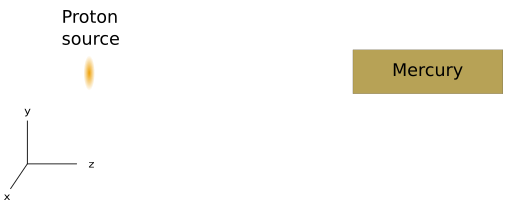
\includegraphics[width=0.60\linewidth]{../figs/mercury.png}
\caption{Planar view of Toy Problem I geometry, 22 cm  x 44 cm x 186 cm }
\label{TPI}
\end{centering}
\end{figure}
Toy problem II (shown in Figure \ref{TPII}) has a rectangular prism enclosing another rectangular
prism. 
The mercury cell has the same dimensions as those of toy problem I. The steel 
cell, which encloses the mercury, is double the size of the mercury cell. 
% Figure
% Figure
\begin{figure}[h!]
\begin{centering}
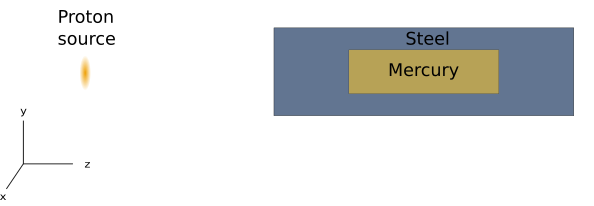
\includegraphics[width=0.70\linewidth]{../figs/mer_steel.png}
\caption{Planar view of Toy Problem II geometry, 44 cm  x 88 cm x 372 cm }
\label{TPII}
\end{centering}
\end{figure}

Both verification problems have a source that models that of the
actual SNS systems. The source is a proton source with energy gaussian dritribution
around 1 GeV. The source is located in a distributed xy plane at z = -256.71 cm, 
where the distribution of the x plane denpends on the y location. 

\subsubsection{Spatial Discretization}
Several superimposed meshes were laid upon Toy Problem I and II. 
The superimposed meshes were 1x1x1, 2x2x2, and 4x4x4. Both toy problems
were also split into 8 equal pieces and 64 equal pieces creating a total of
six distint geometries including the originals. 
Splitting toy problem II into 8 equal cells required some material mixing. 
Each cell in this particular geometry was assigned a steel-mercury mixture
of 3:1. 
This splitting was done in order to compare to the mesh problems. 

\subsection{Workflow to Photon Emissions}
In order to generate the spectrum file, the following steps were carried out:
\begin{itemize}
\item Monte Carlo transport using MCNP 
\item Activation script was run to create the input files for CINDER and  run CINDER
\end{itemize}
A total of 12 problems were run, six for each toy problem. The runs were as follows:
\begin{itemize}
\item Cell rnucs. Mercury cell for Toy Problem I and Mercury and Steel cell for 
Toy Problem II.
\item 1x1x1 uniformly distributed mesh superimposed on the whole problem
\item 2x2x2 uniformly distributed mesh superimposed on the whole problem
\item 4x4x4 uniformly distributed mesh superimposed on the whole problem
\item Geometry split into 8 equal pieces
\item Geometry split into 64 equal pieces
\end{itemize}
Each case was run with 1E6 history particles. 

\newpage
